\section{Results}
Figure~\ref{fig:costheta} shows the distribution of events in $\cos\theta_\text{{sun}}$
for events over the entire energy range of $5$ to $15$\,MeV and the fit to that distribution.\
The fit gives a solar event rate of \InteractionRate\
 and background rate of \BackgroundRate.\
Performing a similar fit in each individual energy bin yielded a best fit solar flux
as a function of energy.\
The fits were combined, in accordance with Eq.~\ref{eq:ll}, yielding an overall best fit flux of
\begin{equation*}
    \Phi_{ES}= 2.53^{+0.31}_{-0.28}\text{(stat.)}^{+0.13}_{-0.10}\text{(syst.)}\times10^6\,\text{cm}^{-2}\text{s}^{-1}\text{.}
\end{equation*}
This value assumes the neutrino flux consists purely of electron flavor neutrinos.\
The result agrees with the elastic scattering flux published by Super-K,
$\Phi_{ES}$=\fluxunits{\SuperKRate}~\cite{superk4}, combining statistical and
systematic errors.\

\figuremacro{residual_plot.pdf}{0.5}{spectrum}{
    (Top) The extracted solar neutrino elastic scattering event rate as a
    function of reconstructed electron kinetic energy $T_{e}$.\
    (Bottom) The same, as a fraction of the expected rate.\
    The red and blue lines show the MC simulation predicted spectrum normalized
    to the best fit flux and the SNO flux measurement~\cite{sno_combined}, respectively.\
    The uncertainty on the SNO result includes reported uncertainty combined with
    mixing parameter uncertainties.\
    The black points are the results of the fits to the $\cos\theta_\text{{sun}}$
    distribution in each energy bin,
    with error bars indicating the combined statistical and systematic
    uncertainty, including energy-correlated uncertainty.\
    A horizontal dash is placed on each error bar indicating the statistics
    only uncertainty; for all points the statistical error is dominant and the systematic
    error bar is not visible above the dash.}

\begin{table}
\begin{center}
\begin{tabular}{l c}
\hline
\hline
Systematic & Effect \\
\hline
Energy Scale & 3.9\% \\
Fiducial Volume & 2.8\% \\
Angular Resolution & 1.7\% \\
Mixing Parameters & 1.4\% \\
Energy Resolution & 0.4\% \\
\hline
Total & 5.0\%\\
\hline
\hline
\end{tabular}
\caption{Effect of each systematic uncertainty on the extracted solar neutrino
         flux. Systematic uncertainties with negligible effects
         are not shown. For asymmetric uncertainties, the larger is shown.}
\label{table:systematics}
\end{center}
\end{table}

Including the effects of solar neutrino oscillations, using the neutrino mixing
parameters given in Ref.~\cite{pdg2016} and the solar production and electron
density distributions given in Ref.~\cite{bs05op} gave a best fit solar flux
of
\begin{equation*}
    \Phi_{\ce{^{8}B}}= 5.95^{+0.75}_{-0.71}\text{(stat.)}^{+0.28}_{-0.30}\text{(syst.)}\times10^{6}\text{cm}^{-2}\text{s}^{-1}\text{.}
\end{equation*}
This result is consistent with the \beight flux as measured by the SNO experiment,
$\Phi_{\ce{^{8}B}}$=\fluxunits{\SNOFlux}~\cite{sno_combined}, combining statistical
and systematic uncertainties.\
Figure~\ref{spectrum} shows the best fit solar neutrino \beight event rate in each
energy bin along with the predicted energy spectrum scaled to the best fit
flux, and scaled to the flux measured by SNO. Each statistical error bar on the
measured rate is affected by both the solar neutrino and background rates in that
energy bin.\
Table~\ref{table:systematics} details how each systematic uncertainty affects this result.\

\begin{figure}[htbp]
    \centering
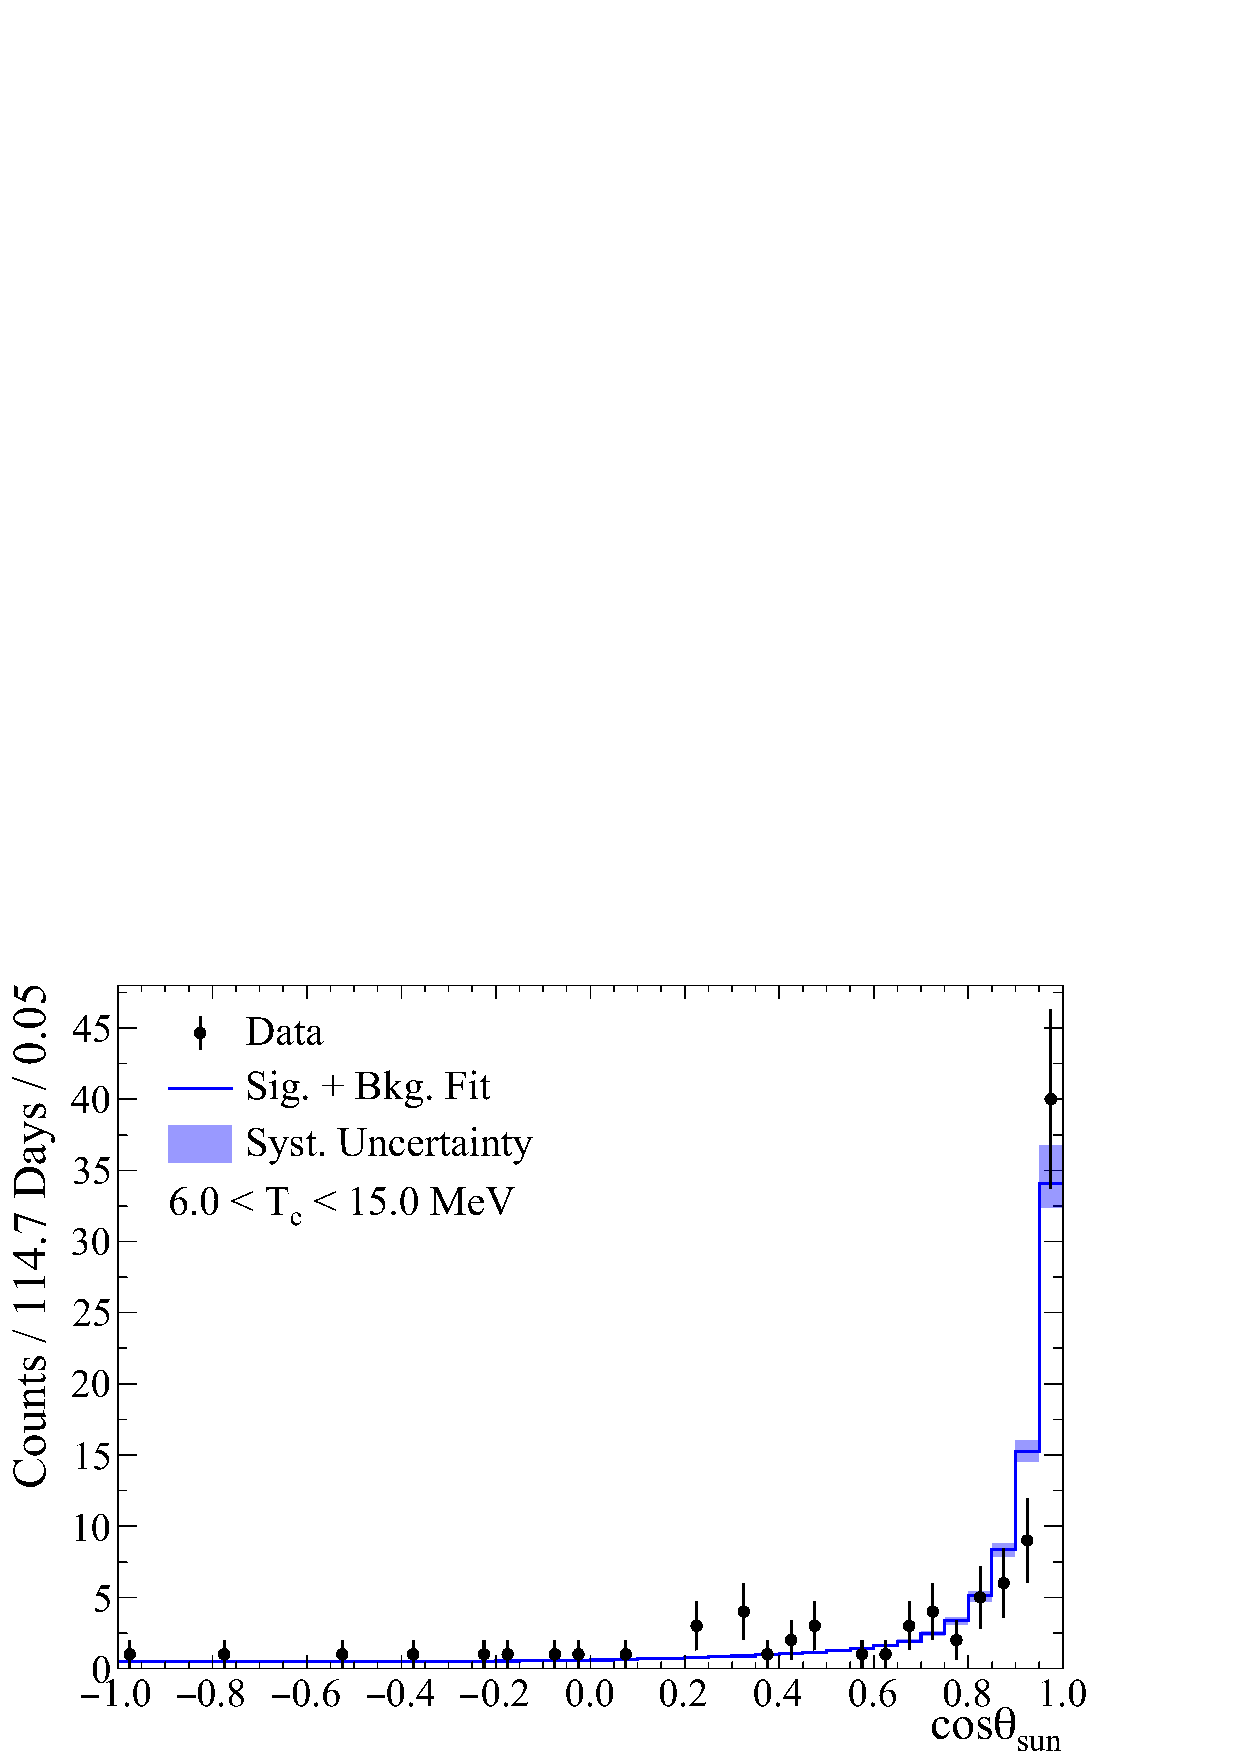
\includegraphics[width=0.5\textwidth]{figures/cos_theta_6mev.pdf}%
\caption{Distribution of event directions with respect to solar direction for
    events with energy in \numrange[range-phrase=--]{6.0}{15.0}\,MeV.}
\label{fig:cos_theta_six}
\end{figure}

The upper five energy bins, \numrange[range-phrase=--]{6.0}{15.0}\,MeV, were an
extremely low background region for this analysis.\
There was very little background contamination from
cosmogenically produced isotopes due primarily to depth of the detector.\
The comparatively high rate of backgrounds in the \numrange[range-phrase=--]{5.0}{6.0}\,MeV bin
comes primarily from decays of radioactive isotopes, such as radon, within the detector.\
Figure~\ref{fig:cos_theta_six} shows the distribution in $\cos\theta_\text{{sun}}$ of events at
energies above 6~MeV, illustrating the low background rate.\
In that energy region the best fit background rate was \LowBackgroundRate, much
lower than the measured solar rate in that energy range, \HighEnergySolarRate.\
For the region above 6~MeV, this is the lowest
background elastic scattering measurement of solar neutrinos in a water
Cherenkov detector.\
